\documentclass[a4paper,12pt]{article}
%\documentclass[a4paper,10pt]{scrartcl}

\usepackage[utf8]{inputenc}
\usepackage[english]{babel}
\usepackage[pdftex]{graphicx}
\usepackage{amssymb}
\usepackage{marvosym}
\usepackage{amsmath}
\usepackage{array}
\usepackage{geometry}

\geometry{verbose,tmargin=1cm,headheight=80pt,lmargin=2cm,bmargin=4cm,rmargin=2.5cm}

\title{Exercise 1 - Solution}
\author{}
\date{}

\pdfinfo{%
  /Title    ()
  /Author   ()
  /Creator  ()
  /Producer ()
  /Subject  ()
  /Keywords ()
}

\begin{document}
\maketitle

\begin{figure}[!ht]
 \centering
 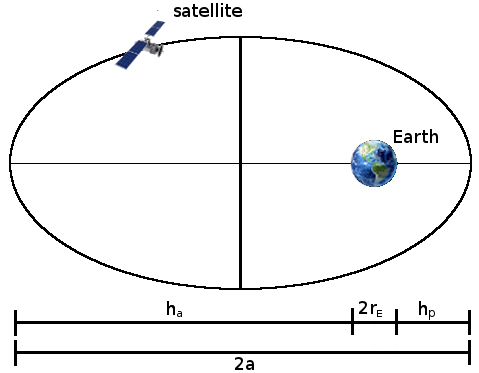
\includegraphics[width=0.6\textwidth]{../Loesungen/pic1}
\end{figure}

\section*{Task 1.1}

given : $T = 106min = 6360s, h_p = 200km, \mu_E = 3.986\cdot 10^5 \frac{km^3}{s^2}, r_E = 6378km$

\noindent to be determined: $h_a$

\[ T = 2\pi\sqrt{\frac{a^3}{\mu_E}} \Rightarrow a = \sqrt[3]{\frac{T^2\mu_E}{4\pi^2}}\]
\[h_a + h_p + 2r_E = 2a \Rightarrow h_a = 2a - h_p - 2r_E = 1882.634... km = 1883km \]


\section*{Task 1.2}

\begin{enumerate}
 \item The satellite has an orbital period of one sideral day, i.e. 23 hours 56 min 4s = 1436.07 min = 1436 min. Since the orbit is circular, the eccentricity is 0.
 \item \[ T = 2\pi\sqrt{\frac{a^3}{\mu_E}} \Rightarrow a = \sqrt[3]{\frac{T^2\mu_E}{4\pi^2}} = 42164.1897... km = 42164 km\]
 \[h = a - r_E = 35786km \]
\end{enumerate}

\section*{Task 1.3}
given : $h_a = 320km, h_p = 270km, \mu_E = 3.986\cdot 10^5 \frac{km^3}{s^2}, r_E = 6378km$

\noindent to be determined: a, $\varepsilon$

\[ 2a = h_a + h_p + 2r_E \Rightarrow a = \frac{h_a + h_p + 2r_E}{2} = 6673km \]
\[ T = 2\pi\sqrt{\frac{a^3}{\mu_E}} = 5424.91..s = 90.415min = 90 min\]
\[h_p + r_E = a(1-\varepsilon) \Rightarrow \varepsilon = 1 - \frac{h_p + r_E}{a} = 0.0037 \Rightarrow \text{almost circular}\] 

\section*{Task 1.4}
given : $T = 225 \text{ earth days} = 225\cdot 86400s, \mu_S = 1.327\cdot 10^{11} \frac{km^3}{s^2}$

\noindent to be determined: $a$

\[ a = \sqrt[3]{\frac{T^2\mu_S}{4\pi^2}} = 1.083 \cdot 10^8 km = 108 \text{ million km} \]

\section*{Task 1.5}
given : $T = 6.5 \text{ years} = 6.5\cdot365\cdot24\cdot3600 s, \mu_S = 1.327\cdot 10^{11} \frac{km^3}{s^2}, h_p = 185\cdot 10^6 km, r_S = 695,800 km$

\noindent to be determined: $a, \varepsilon, v_{min}, v_{max}, \Phi$
\begin{enumerate}
 \item \[ a = \sqrt[3]{\frac{T^2\mu_S}{4\pi^2}} = 5.20775... \cdot 10^8 km = 521 \text{ million km} \]
 \item \[ h_p + r_E = a(1-\varepsilon) \Rightarrow \varepsilon = 1 - \frac{h_p + r_S}{a} = 0.643578 = 0.64 \]
 \item \[ v_{max} = \sqrt{\mu_S\bigg(\frac{2}{h_p+r_S} - \frac{1}{a}\bigg)} = 34.2640... \frac{km}{s} = 34.26 \frac{km}{s} \]
 \[ h_a = 2a - 2r_S -h_p = 853,608,400 = 854 \text{ million km} \]
 \[ v_{min} = \sqrt{\mu_S\bigg(\frac{2}{h_a+r_S} - \frac{1}{a}\bigg)} = 7.4383 \frac{km}{s} = 7.44 \frac{km}{s}\]
 \item formula from lecture: 
 \[r = a\frac{1-\varepsilon^2}{r\varepsilon cos(\Phi)}\]
 \[\Rightarrow \text{true anomaly } \Phi = arccos(a\frac{1-\varepsilon^2}{r^2\varepsilon})\]
\end{enumerate}



\end{document}
